\documentclass[12pt, titlepage, a4paper]{article}
\usepackage[utf8]{inputenc}
\usepackage{graphicx}

\begin{document}
	\title{Flappa Freqt}
	\author{Cecilia Lagerwall - cecla125 \\ Daniel Rönnkvist - danro716 \\
			Therese Komstadius - theko867 \\ \\ Linköpings universitet}
	\date{2014-10-10}
	\maketitle
  \renewcommand*\abstractname{Sammanfattning}
  \begin{abstract}
		flappa för fan
	\end{abstract}
	\section{Inledning}
		I denna rapport redovisas projektet “Flappa Freqt” som genomfördes i kursen Ljudfysik, TFYA65, ht 2014 vid Linköpings universitet. Syftet med projektet var att skapa ett spel där spelaren kontrollerade spelet med hjälp av rösten.
	\section{Bakgrund}
		Eftersom projektet skulle avhandla ljudfysik blev det tidigt bestämt att fokus skulle ligga på att uppta och omvandla ljud. Därför baserades grundiden för spelet på ett redan existerande koncept. Konceptet som valdes var det bakom spelet “Flappy bird”, med skillnaden att olika röstfrekvenser skulle förlytta spelobjektet i vertikalled. Det beslutades även att spelet skulle utvecklas för en enhet med inbyggd mikrofon, därför valdes Javascript som programmeringsspråk för att utveckla till en webbläsare. Javascript valdes även för att det skulle vara enklare att hitta ett färdigt spelskelett.
	\section{Metod}
		\subsection{Verktyg}
			För att alla skulle kunna jobba tillsammans med samma kod och samtidigt hålla den strukturerad valdes versionshanteringssystemet Git. Detta med hjälp av GitHub underlättade arbetet.
			\\ \\
			För att uppta ljud från mikrofonen i en webbläsare användes \textit{Web Audio API}\cite{MDN} som är ett API, \textit{application programming interface}, för Javascript. Med hjälp av detta interface kunde en ström från mikrofonen (i det här fallet på en dator) skapas och ljudet kunde sparas och bearbetas i realtid.
		\subsection{Tillvägagångssätt}
			För att inte behöva bearbeta ljudet i hela frekvensomfånget(0-20 000 Hz) applicerades ett bandpassfilter på ljudströmmen. Bandpasset valdes att vara mellan 150 och 1500 Hz, detta för att den mänskliga rösten ligger mellan dessa två frekvenser\cite{freq}.
			\\ \\
			För att analysera ljudet sparades alla inspelade frekvenser i en buffert. Bufferten loopades sedan igenom för att hitta den frekvens med högst amplitud. Från detta amplitudvärde subtraherades ett bestämt tröskelvärde för att hitta en gränsnivå. De frekvenser som låg över denna gräns summerades och den totala summan dividerades med antalet summerade frekvenser för att få fram en medelfrekvens. (Se bild 1.) Eftersom ljudet från mikrofonen samplades med 1024 sampel/frekvensomfång över ett 20 000 Hz omfång multiplicerades medelfrekvensen med 19.5 (1) för att få fram det riktiga frekvensvärdet.
			\begin{figure}[h!]
				\centering
					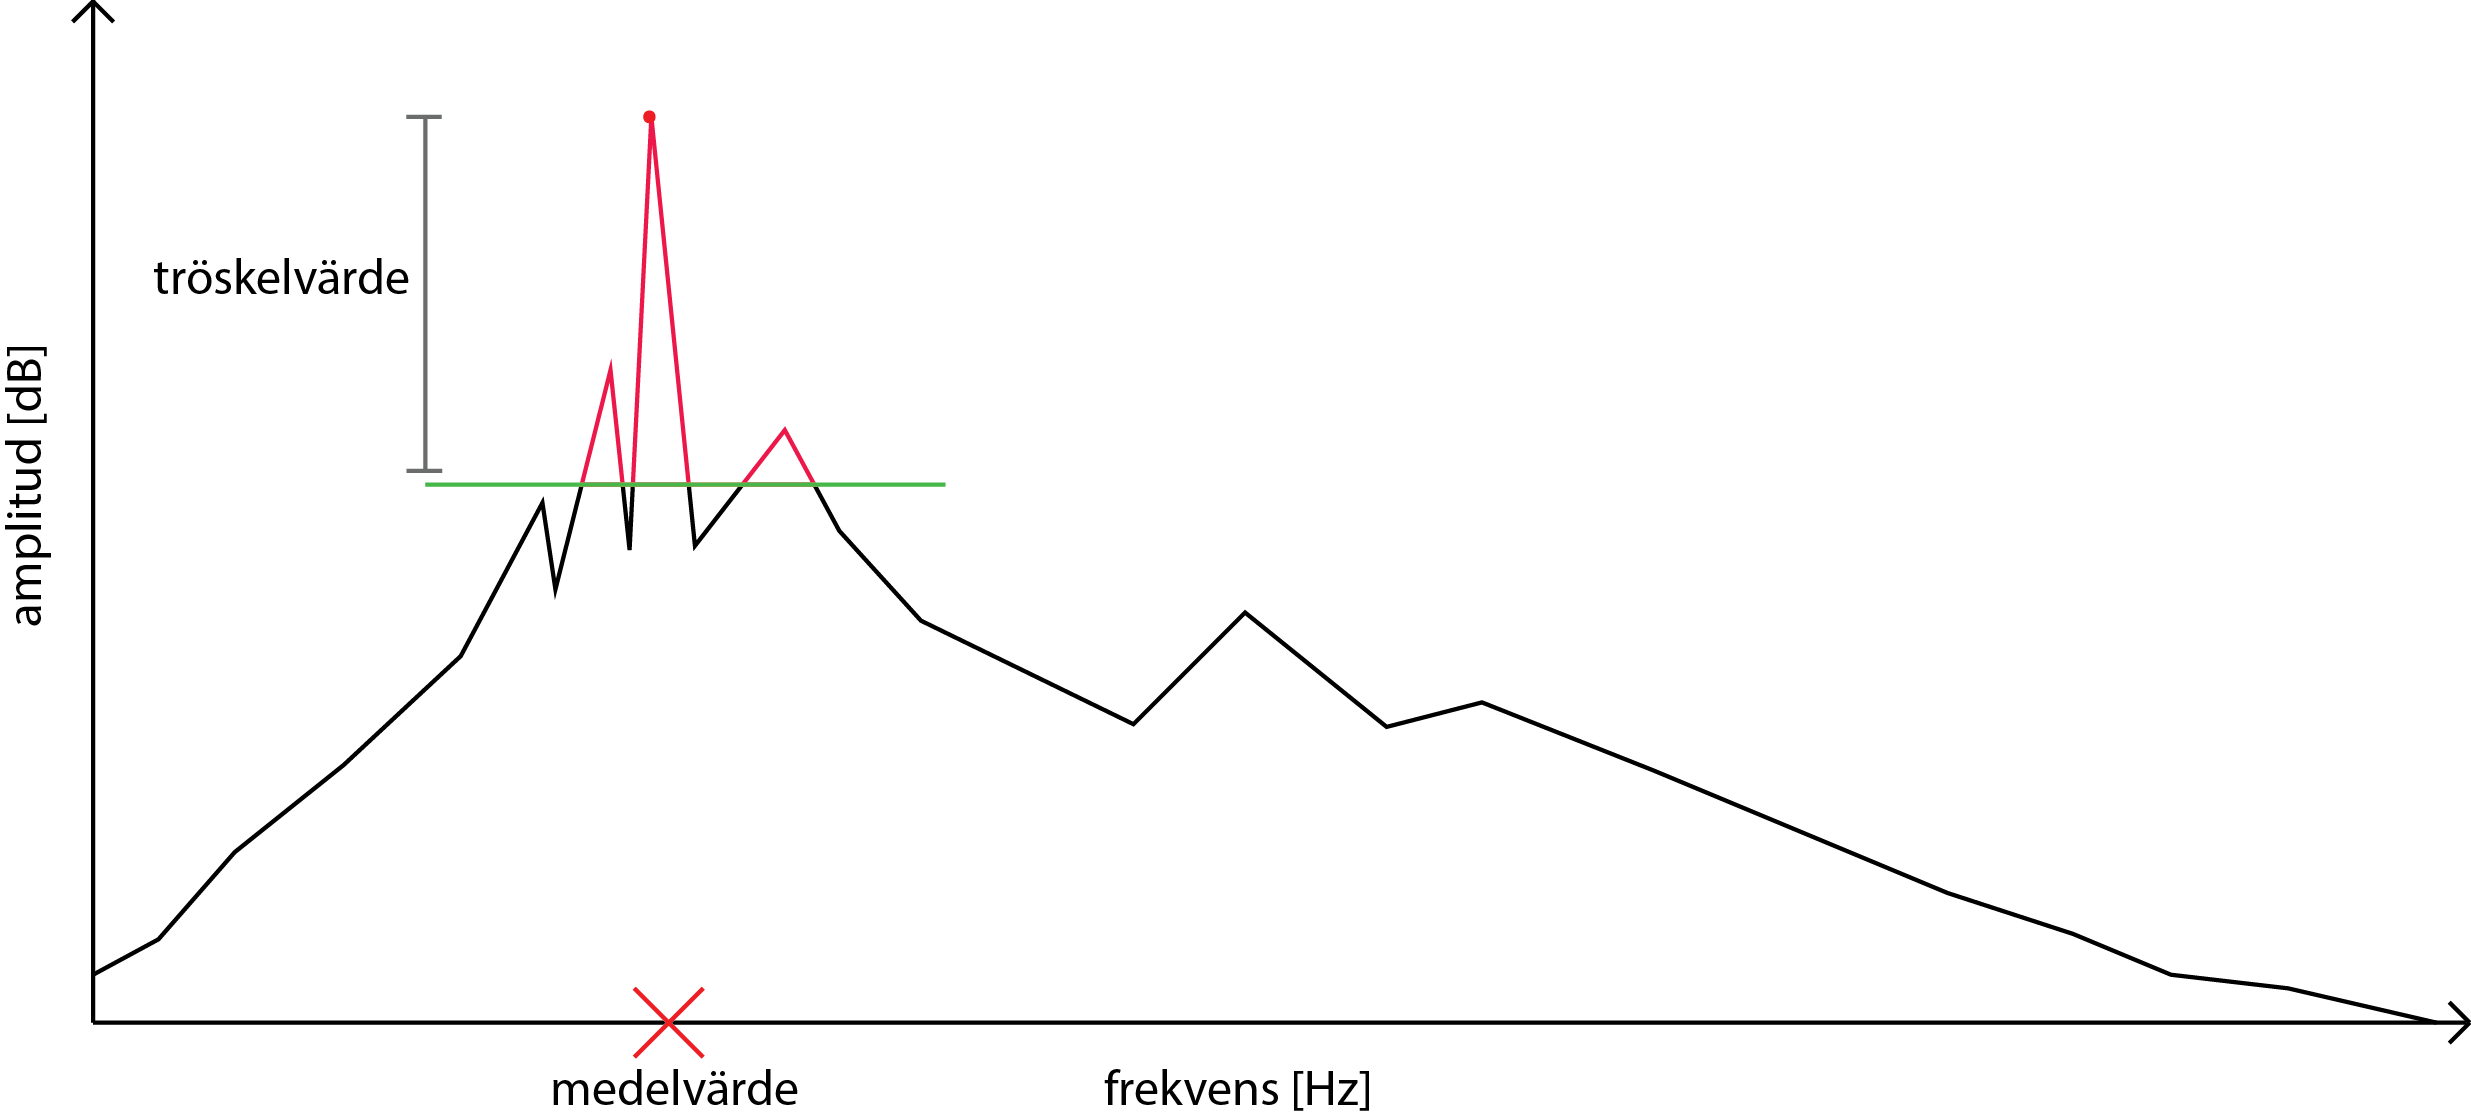
\includegraphics[width=1\textwidth]{explanation.png}
  						\caption{En illustration som förklarar hur medelfrekvensen beräknas.}
			\end{figure}

	\section{Resultat}
	\section{Diskussion}
	\section{Slutsats}
	\section{Referenser}
	\renewcommand{\addcontentsline}[3]{}% Remove functionality of \addcontentsline
  \renewcommand{\section}[2]{}% Remove functionality of \section
  \begin{thebibliography}{1}
  \bibitem{MDN}
    Mozilla Developer Network.
    \emph{Web Audio API.}
    https://developer.mozilla.org/en-US/docs/Web/API/Web\_Audio\_API, 2014-10-07
  \bibitem{freq}
    Befria Samtalet.
    \emph{Fakta om ljudmiljö.}
    http://www.befriasamtalet.se/fakta
  \bibitem{AnalyserNode}
    Mozilla Developer Network.
    \emph{AnalyserNode.}
    https://developer.mozilla.org/en-US/docs/Web/API/AnalyserNode
  \end{thebibliography}
  \section{Bilagor}
  Koden för projektet: https://github.com/danielronnkvist/flappy-wueeaaaoooo

\end{document}
